\ref{chap:reinforcement}% -*- root: ../main.tex -*-
\chapter{Uczenie ze wzmocnieniem}
\label{chap:reinforcement}

W przeszłości było wiele prób zbudowania przeróżnych kognitywnych architektur. Miały one tworzyć unifikujący obraz działania mózgu lub oddawać w jakiś sposób jego działanie. Te modele były często luźno inspirowane pewnymi spostrzeżeniami na temat funkcjonowania mózgu i były nastawione na przybliżenie generalnych metod jego działania. Zazwyczaj takie modele wymagały także ogromnych zbiorów stwierdzeń na temat świata w duchu symbolicznego AI. My co prawda w rozdziale o symbolicznym AI skupiliśmy się na może pobocznym temacie, jakim są drzewa poszukiwań, ale w tym dziale często korzysta się ze stwierdzeń zapisanych w formie logiki, tak jak to powiedzieliśmy na początku tamtego rozdziału. Takie symboliczne podejście ma swoje plusy, wykorzystuje, chociażby aparat matematyczny do określania wartości stwierdzeń jest jednak zbyt sztywne dla większości rozwiązań. Sam spróbuj zapisać informacje na jakiś temat za pomocą samych stwierdzeń, żeby przekonać się, że nie jest to łatwe zadanie. Tak więc systemy te wymagały ogromnych zbiorów twierdzeń. Działo się tak, ponieważ te systemy nie posiadały własnego mechanizmu interpretacji tego, co dzieje się w świecie i wyciągania z tego wniosków. Można powiedzieć, że pod pewnymi względami te systemy były nawet w tyle za robotem Shakey, który potrafił interpretować swój prosty świat. Niektóre takie projekty zużyły tysiące godzin pracy wolontariuszy, żeby zwiększyć pojemność baz danych na temat świata, z nadzieją, że jeśli uchwycą ich wystarczającą ilość, to te systemy będą mogły rozumować jak ludzie. Okazuje się, jednak że nikt nie mówi nam nigdy, co się stanie, jeśli będziemy biec ulicą z pełnym wiadrem wody, a jednak wiemy, że nasze nogi będą mokre. Z tego i innych powodów, miliony relacji później ten wysiłek zdaje się bezowocny. Ignorowanie motywacji, uczuć, emocji i stanów umysłu mogło być fundamentalnym powodem porażki tych wysiłków. Jest jednak bardziej podstawowy problem z takim podejściem. Tworzenie dużego systemu z wielu wcześniej zdefiniowanych zasad nie jest proste ze względu na występujące między nimi interakcje. Wyobraź sobie, że próbujesz zbudować samochód od podstaw, nie wiedząc nawet jakie systemy i funkcjonalności powinny zostać dodane. Ta metafora oddaje bezsens próby skonstruowania kopii mózgu od podstaw bez posiadania planu. To podejście nie pozwala na testowanie części przed dodaniem ich do większego systemu i nieprawidłowe działanie jednej z nich oznacza, że całość nadaje się do wyrzucenia, ponieważ nie wiemy która część jest odpowiedzialna za niepowodzenie. Pracując obok tych wysiłków byli naukowcy tacy jak Richard Sutton, którzy próbowali odkryć podstawowe zasady kierujące zachowaniem inteligentnych systemów. Powzięli oni podejście matematyczne, patrząc się na umysł tylko w celu inspiracji. Te wysiłki okazują się dzisiaj dużo bardziej skuteczne. Niektóre z nich zdają się nawet wyjaśniać niektóre zjawiska występujące w naszej czaszce, jak np. uczenie TD, które zostało połączone z działaniem systemu dopaminergicznego. Dużą przewagą tego podejścia jest również to, że uczenie ze wzmocnieniem, ponieważ używa pewnych pojęć występujących w innych dziedzinach sztucznej inteligencji, może być dość łatwo połączone do innych odkryć takich jak sieci neuronowe. To oferuje efekt synergii i łatwość konceptualną.

\section{Problem uczenia ze wzmocnieniem}

Jak jednak możemy zdefiniować działanie całego inteligentnego systemu, jakim jest nasz mózg za pomocą kilku prostych zasad? Uczenie ze wzmocnieniem (ang. reinforcement learning albo RL w skrócie) identyfikuje kilka niezbędnych składników koniecznych dla inteligentnego zachowania. Na początek potrzebujemy pewnych informacji koniecznych, żeby podjąć decyzję. Ta właściwość jest nazywana \textbf{stanem}. Następnie potrzebujemy aktora. Aktor jest osobą, zwierzęciem, robotem, który używa informacji o stanie, żeby podejmować decyzje. Aktor otrzymuje \textbf{nagrodę} po każdej zmianie stanu lub po pewnej serii stanów. Nagroda jest podobna do zjawiska przyjemności i bólu, tak więc aktor lubi zwiększać ilość nagrody. Ostatecznie aktor może podejmować pewne \textbf{akcje} które wpływają w jakiś sposób na stan. Te akcje mogą być: przesunięciem bierki w szachach, kierunek ruchu ramienia robota lub może wybranie problemu, nad którym powinno się pracować. Ten proces może być zwizualizowany jako pewnego rodzaju okrąg, w którym informacje płyną od środowiska do aktora i do aktora do środowiska. Akcje aktora są modyfikowane przez napływający sygnał nagrody.\newline

\noindent Są jeszce dwa inne kluczowe elementy problemu RL. Tak zwany \textbf{zbiór zasad} (ang. policy) jest pierwszą z nich. Zbiór zasad określa dla każdego stanu akcje, które zostaną podjęte przez aktora. Tak więc można myśleć o zbiorze zasad, jak o wyniku działania mózgu.

\begin{equation}
p(s|a)
\end{equation}

\noindent Zbiór zasad $\boldsymbol{p}$ dla danego stanu $\boldsymbol{s}$ przy podjęciu akcji $\boldsymbol{a}$.\newline

\clearpage
\begin{figure}[H]
\centering
\includepdf[pages=19]{mputo.pdf}
\caption{Problem uczenia ze wzmocnieniem}
\end{figure}
\clearpage

\noindent Możemy też zidentyfikować funkcję wartości. Poprzednio mówiliśmy o funkcji wartości, ale dla problemu RL możemy określić pewne jej dodatkowe właściwości. Funkcja wartości jest sumą wszystkich sygnałów nagrody od teraz od ostatniego występującego stanu. Możemy to zapisać jako:

\begin{equation}
v(a, a_1, a_2, ...) = \Sigma(r_i, r_{i+1}, r_{i+2}, …)
\end{equation}

\noindent Gdzie $\boldsymbol{v}$ jest funkcją wartości, $\boldsymbol{a_n}$ są akcjami, które podejmuje aktor, a $\boldsymbol{r_n}$ jest sygnałem nagrody w kroku $\boldsymbol{n}$. Ważne jest, żeby zobaczyć, że chcielibyśmy znać funkcję wartości, ponieważ powiedziałaby nam ona, ile nagrody otrzymamy w przyszłości.


\section{Wieloręczny bandyta}

Wyjaśniliśmy, że całe myślenie aktora może być podsumowane jako zbiór zasad. Jeśli znalibyśmy optymalny zbiór zasad, to moglibyśmy osiągnąć najwyższe możliwe nagrody od teraz do końca wszechświata. Problemem jest jednak to, że większość aktorów wie, na początku, bardzo mało o funkcjonowaniu środowiska, w którym się znajdują, więc nie są w stanie powiedzieć, co jest dla nich najkorzystniejsze. Co powinien zrobić taki aktor, żeby stać się lepszym w poszukiwaniu nagrody? Wyobraź sobie bycie w ogromnym kasynie, gdzie znajduje się wiele automatów do gier zwanych powszechnie jednoręcznymi bandytami (prawdopodobnie dlatego, że każdy, kto wchodzi w bliski kontakt z taką maszyną, zostaje ograbiony). W tym kasynie jest wiele różnych maszyn, każda dająca inną spodziewaną wygraną. My chcemy znaleźć taką, która da nam wygrać lub nie przegrać, jak największą ilość pieniędzy. Może brzmi to tylko jak ładna metafora, ale tak opisany problem nazywany jest problemem \textbf{wieloręcznego bandyty} (ang. multi-armed bandit). Zastanówmy się teraz nad najlepszą strategią działania w takim kasynie. Na początku nic nie wiemy o maszynach, także konieczne jest, żebyśmy dokonali pewnej ilości eksploracji, to znaczy, że koniecznym jest aby pociągnąć wajchy należące do wielu jednoręcznych bandytów w poszukiwaniu takiego, który daje dobre nagrody. W ten sposób możemy znaleźć najbardziej opłacalną maszynę, ale jeśli tylko eksplorujemy, to nie otrzymamy korzyści wynikających z wykorzystania takiej maszyny, czyli eksploatacji. Strategia, która zawiera te dwie korzyści, czyli eksplorację i eksploatację nazywana jest \textbf{epsilon-chciwa} (ang. epsilon greedy). Określa ona, że powinniśmy eksplorować przez $\boldsymbol{e}$ ilość czasu i eksploatować to, czego się nauczyliśmy przez $\boldsymbol{1-e}$ ilość czasu. Używając strategii epsilon-chciwej, będziemy otrzymywać wyższe nagrody, wraz z tym, jak będziemy się stawać lepsi w danym zadaniu. Wynika to oczywiście z faktu, że wykonujemy co jakiś czas fazę eksploatacji, w ciągu której wykorzystujemy najlepszy automat. Jak ustalić przez ile czasu powinno się to jednak odbywać? Zazwyczaj ustawilibyśmy $\boldsymbol{e}$ tak, żeby równała się pewnej małej wartości takiej, jak $\boldsymbol{e}$=0.1. To oznacza, że eksplorujemy przez tylko 10\% czasu. W długim okresie wystarczy to jednak do znalezienia optymalnego rozwiązania. Jednym problemem tego podejścia jest to, że nawet jeśli znamy spodziewaną wartość każdej z maszyn z wielką dokładnością, to nadal będziemy zmuszeni poświęcać 10\% czasu na eksplorowanie, co będzie nas powstrzymywać przed otrzymaniem najwyższej możliwej nagrody. Tu pojawia się modyfikacja strategii epsilon-chciwej. W niej będziemy zmniejszać $\boldsymbol{e}$ po pewnej ilości $\boldsymbol{N}$ prób. Za każdym razem, gdy wykonaliśmy wielokrotność $\boldsymbol{N}$ prób zmniejszymy epsilon, używając równania:

\begin{equation}
e = y * e
\end{equation}

\noindent Gdzie $\boldsymbol{y}$ jest pewną wartością pomiędzy 0 a 1.\newline

To pozwoli nam wykonywać mniej i mniej eksploracji, w miarę tego, jak stajemy się lepsi w wykonywaniu zadania, jednocześnie zwiększając naszą nagrodę albo jak w przypadku jednoręcznych bandytów – zyski. Jest jeszcze jedna rzecz, którą moglibyśmy zrobić. Jeśli znamy najwyższą możliwą wartość funkcji wartości, to możemy zmniejszać parametr $\boldsymbol{e}$ proporcjonalnie do poprawy w funkcji wartości. Jest to pewnego rodzaju strategia równoważenia ilości eksploracji z wielkością funkcji wartości. To pozwoli nam przeznaczać na eksplorację ilość czasu równą procentowi nieosiągniętej maksymalnej wartości. Jeśli funkcja wartości osiągnęła np. 30\%, to eksplorujemy przez 70\% czasu. Kiedy poprawimy się, w tym co robimy, to zmniejszymy ilość eksploracji, bo będzie ona mniej korzystna, jako że częściowo wiemy już jak osiągać pewien procent wartości. Przed wprowadzeniem jeszcze jednego sposobu powtórzmy to, czego już się nauczyliśmy, a mianowicie, że funkcja wartości jest zdefiniowana jako:

\begin{equation}
v(a, a_1, a_2, ...) = \Sigma(r_i, r_{i+1}, r_{i+2}, …)
\end{equation}

\noindent Podane równanie, żeby otrzymać funkcję wartości, sumuje wszystkie nagrody od teraz do nieskończoności z równą wagą. Jednak w prawdziwym życiu troszczymy się dużo bardziej o nagrodę w momencie $\boldsymbol{r_i}$ niż tą w momencie $\boldsymbol{r_{i+1000}}$ Dlaczego tak się dzieje? Jednym z powodów jest zapewne fakt, że przyszłość nie jest tak pewna, jak teraźniejszość, więc z chęcią zamienimy nagrodę daleko na horyzoncie na mniej oddaloną, bo ta odległa może nigdy nie nadejść. Dlatego powinniśmy dodać pewien parament określający pewność co do przyszłości. Nazwijmy go $\boldsymbol{d}$ tak jak we współczynniku dyskontowym. Pomnóżmy $\boldsymbol{r_{i+1}}$ przez $\boldsymbol{d}$, $\boldsymbol{r_{i+2}}$ przez $\boldsymbol{d * d}$, $\boldsymbol{r_{i+3}}$ przez $\boldsymbol{d * d * d}$ itd.

\begin{equation}
v(a, a_1, a_2, ...) = \Sigma(r_i, r_{i+1} * d, r_{i+2} * d^2, …)
\end{equation}

To jest bardziej realistyczny pogląd na naszą funkcję wartości. Teraz pamiętając o tym, możemy stworzyć sieć neuronową, która będzie przybliżać tę funkcję wartości. Mając tę sieć, będziemy eksploatować wieloręcznego bandytę, używając sieci neuronowej do aproksymacji jakości każdego jednoręcznego bandyty. To podejście jednak nie zadziała, ponieważ nie daliśmy naszej sieci żadnych przykładów do trenowania. Dlatego nadal potrzebujemy eksplorować, żeby uzyskać przykłady, na których będziemy trenować. Wytrenujemy taką sieć, podając przykłady sytuacji, które napotkaliśmy i odpowiadającą im sumę nagród jak pokazano wyżej. Żeby wybrać pomiędzy stanem eksploracji i eksploatacji, użyjemy formuły UCT takiej jak w podrozdziale 4.6 dotyczącym MCTS. Dla każdego "bandyty" obliczymy i wybierzemy tego z najwyższą wartością:

\begin{equation}
UCB1 = v + c * \sqrt{ln(N) / n}
\end{equation}

\noindent Gdzie $\boldsymbol{v}$ będzie rezultatem otrzymanym z naszej sieci, $\boldsymbol{c}$ stałą eksploracji, $\boldsymbol{N}$ całkowitą liczbą prób, a $\boldsymbol{n}$ ilością prób wykonanych na konkretnym automacie.

\clearpage
\begin{figure}[H]
\centering
\includepdf[pages=20]{mputo.pdf}
\caption{Wieloręczny bandyta}
\end{figure}
\clearpage

\section{MDP}

Łańcuch Markowa jest modelem środowiska, w którym następny stan zależy tylko od obecnego stanu i od prawdopodobieństwa zmiany tego stanu. Z tego powodu jest nazywany procesem stochastycznym. Wyobraźmy sobie, dla przykładu, przewidywanie pogody. Nasz model może pokazywać, że jeśli mamy ładną pogodę to występuje 7\% szansy na to, że jutro będzie padać. Jeśli jednak już dzisiaj pada, to występuje 13\% szansy, że pojawi się burza, 36\% szansy, że jutro też będzie padać i 51\% szans, że jutro się rozpogodzi. Taki model jest właśnie nazywany łańcuchem Markowa. Może on się jednak składać z wielu więcej stanów i przejść między nimi. Możemy zaprezentować taki model graficznie jako graf z węzłami stanu połączonymi krawędziami związanymi z prawdopodobieństwem.

\begin{equation}
(S, P)
\end{equation}

\noindent $\boldsymbol{S}$ jest stanem, $\boldsymbol{P}$ jest prawdopodobieństwem zmiany stanu.\newline

\noindent \textbf{Problem decyzyjny Markowa} (ang. Markov decision process, MDP dla krótkości zapisu) jest rozszerzeniem pomysłu łańcucha Markowa, które dodaje akcje i nagrody. Ten model jest wyjątkowo podatny na idee uczenia ze wzmocnieniem. W MDP mamy stany, które prowadzą z pewnym prawdopodobieństwem do akcji, które znów prowadzą z innymi prawdopodobieństwami do pewnych stanów. Każda zmiana stanu związana jest z nagrodą. Rozszerzmy nas przykład dot. pogody o jej przewidywanie. Powiedzmy, że jeśli jest ładna pogoda i poprawnie przewidzimy, że jutro też będzie ładna, to otrzymujemy nagrodę +1. Jeśli jednak przewidzimy, że będzie ładnie, a w rzeczywistości będzie padać, to otrzymujemy nagrodę -2. Następnie przechodzimy do kolejnego stanu, w zależności od tego, co rzeczywiście się stało i tak, jeśli trafimy np. na deszcz, to otrzymujemy nagrodę -2, przesuwamy się do węzła z deszczem. Teraz mamy 3 przewidywania: ładna pogoda, deszcz, burza. Jeśli przewidzimy ładną pogodę, to otrzymujemy +2, jeśli to samo zrobimy z deszczem to +3, jeśli przewidzimy burzę +5. Jednak jeśli nie uda się nam przewidzieć sytuacji, to otrzymamy -1 za źle przewidzianą ładną pogodę, -2 za deszcz i -5 za burzę. Następnie przechodzimy do kolejnego węzła, według tego, co naprawdę się wydarzyło. Jeśli zdarzyła się akurat burza, to kończymy, bo od burzy, w naszym przykładzie, nie prowadzą żadne strzałki. Oznacza to, że jest ona węzłem końcowym.

\begin{equation}
(S, A, P, R)
\end{equation}

\noindent $\boldsymbol{S}$ jest stanem, $\boldsymbol{P}$ jest prawdopodobieństwem zmiany stanu, tak jak w łańcuchu Markowa, $\boldsymbol{A}$ są akcjami, które aktor może wybrać, a $\boldsymbol{R}$ są nagrodami związanymi z przeszłym i obecnym stanem.

\clearpage
\begin{figure}[H]
\centering
\includepdf[pages=24]{mputo.pdf}
\caption{Przykładowe przejścia między stanami MDP}
\end{figure}
\clearpage

\section{Uczenie Monte-Carlo}

Jedną z metod uczenia zbioru zasad oraz funkcji wartości jest \textbf{uczenie Monte-Carlo}. Działa ono poprzez patrzenie się jaką kumulatywną nagrodę następującą po stanie $\boldsymbol{s}$ otrzymał aktor. Jest to niedokładne przybliżenie funkcji wartości. Jak pamiętamy, suma wszystkich nagród jest równa funkcji wartości. Mogłoby się nam wydawać, że suma nagród będzie dokładnie odzwierciedlać funkcję wartości i możemy uczyć na tych pojedynczych przykładach z powodzeniem. Tak jednak nie jest, ponieważ po nastąpieniu wydarzenia, które śledzimy, następują też inne wydarzenia, które mają wpływ na wynik sumy nagród. Dlatego bierzemy średnią z wielu takich wydarzeń, aby otrzymać przybliżony wynik funkcji wartości. Jeśli weźmiemy wiele przykładów to wydarzenia następujące po naszym wydarzeniu, którym jesteśmy zainteresowani, się uśrednią. To sprawi, że przewidywanie będzie bliższe rzeczywistej oczekiwanej wartości wydarzenia. Dodawanie kolejnych przykładów do naszego przewidywania na temat jednego wydarzenia daje nam lepsze i lepsze prognozy na temat rzeczywistej funkcji wartości. Jest jednak pewien problem z tym podejściem. Chodzi tu o sposób sumowania nagród. Jak możemy zsumować niekończące się nagrody? Jednym z problemów uczenia Monte-Carlo jest to, że historia potrzebuje mieć punkt końcowy. Dzieje się tak, ponieważ nie możemy sumować nieskończonej liczby nagród bez ucinania reszty w jakimś arbitralnym punkcie, żeby być w stanie nauczyć się czegokolwiek.

\begin{equation}
v(s) = AVG(v_1, v_2, v_3, …)
\end{equation}

\noindent Uczenie Monte-Carlo, gdzie $\boldsymbol{v_1}$, $\boldsymbol{v_2}$ itd. są sumami nagród w konkretnym epizodzie, a $\boldsymbol{v}$ jest funkcją wartości otrzymaną przez wzięcie średniej z tych sum.\newline

Powiedzmy, jak moglibyśmy zaimplementować uczenie Monte-Carlo. Możemy sobie wyobrazić posiadanie wielkiej tablicy z osobnym rekordem dla każdego stanu $\boldsymbol{s}$. W każdej komórce umieszczalibyśmy tą średnią. Teraz, aby aktualizować wartość każdej z tych komórek, potrzebujemy zasady aktualizacji. Moglibyśmy ją otrzymać, utrzymując w pamięci dwie informacje: jedną z sumą wszystkich nagród w różnych epizodach i drugą z ilością epizodów, które sprawdziliśmy. Dzieląc pierwszą wartość przez drugą, otrzymalibyśmy wynik. Jest jednak inna metoda dająca ten sam wynik:

\begin{equation}
u_{avg} = \frac{x + (k - 1) * u_{oldAvg}}{k}
\end{equation}

\noindent Gdzie $\boldsymbol{u_{avg}}$ jest nową średnią, $\boldsymbol{u_{oldAvg}}$ bieżącą średnią, $\boldsymbol{k}$ jest liczbą epizodów, a $\boldsymbol{x}$ jest nowym przykładem sumy nagród, który napotkaliśmy.\newline

\clearpage
\begin{figure}[H]
\centering
\includepdf[pages=23]{mputo.pdf}
\caption{Rozwinięcie Monte-Carlo}
\end{figure}
\clearpage

To podejście jest możliwe dla małych problemów, jednak kiedy problem rośnie do dużych rozmiarów, jak na przykład podczas gry w szachy, staje się niemożliwym, aby utrzymywać rekord każdego możliwego stanu. Jak moglibyśmy przybliżyć działanie takiej tablicy? Tu na pomoc przychodzi generalna \textbf{aproksymacja funkcji}. W naszym przypadku użyjemy jednego z aproksymatorów jakim jest sieć neuronowa. Sieci neuronowe są tak nazywane, ponieważ w teorii mogą reprezentować każdą możliwą funkcję z pewną dokładnością. Tak więc będziemy używać sieci neuronowej do aproksymowania działania tabeli przeglądowej. Jakie będzie wejście, wyjście i nagroda dla naszej sieci? Wejściem będzie stan. Wyjście określimy jako wartość funkcji wartości dla danego stany wejściowego. Tak np. wejściem może być pozycja szachowa, a wyjściem numeryczna ocena pozycji przez arcymistrza szachowego. Żeby przybliżać wynik otrzymywany przez propagację przez sieć, do oceny profesjonalisty, użyjemy funkcji wartości, która będzie używać różnicy między wyjściem a sumą nagród dla danego epizodu do swojego uczenia. Następnie odejmiemy ocenę profesjonalisty od oceny sieci i wszystko to podniesiemy następnie do kwadratu. Taka funkcja nazywana jest \textbf{średnim błędem kwadratowym} (ang. mean squared error lub MSE).

\begin{equation}
MSE = (u_{expected} - u_{net})^2
\end{equation}

\noindent $\boldsymbol{U_{expected}}$ jest sumą nagród albo funkcją wartości dla naszego epizodu, $\boldsymbol{u_{net}}$ jest wyjściem naszej sieci neuronowej. Musimy tylko pamiętać, że jeśli nasz epizod jest nieskończony, będziemy musieli w pewnym momencie uciąć resztę nagród.\newline

Taka funkcja wartości zapewni nam dobre uczenie ze względu na to, że kara, jaką będzie otrzymywać sieć, będzie zależeć od odległości między oceną sieci a oceną spodziewaną. Zamiast oceny profesjonalisty możemy wziąć wynik gry, co jest bardziej realne, ponieważ zazwyczaj nie mamy zbioru pozycji ocenionych przez profesjonalistę. Jeśli tak właśnie jest, to możemy wziąć jak największą liczbę rozegranych gier z ich wynikami. Wybrać spośród nich pewną liczbę pozycji z wynikami i na takiej podstawie uczyć naszą sieć. Zauważmy, że popularne pozycje takie jak np. 1.e4 2.e5 mogą się powtórzyć w naszym zbiorze wielokrotnie. Na dodatek mogą mieć one różne wyniki, ponieważ niektórzy gracze mogli wygrać a inni przegrać z tej samej pozycji. Nie przeszkadza to jednak w uczeniu, ponieważ sieć tak jak wcześniej tablica uśredni te wyniki.

\clearpage
\begin{figure}[H]
\centering
\includepdf[pages=22]{mputo.pdf}
\caption{Propagacja błędu w TD}
\end{figure}
\clearpage

\section{Uczenie TD}

Alternatywą dla metody Monte-Carlo jest metoda \textbf{temporalnych różnic} (ang. temporal difference, TD dla krótkości zapisu). W metodzie TD szukamy różnic pomiędzy funkcją wartości dla następujących po sobie stanów. Wyobraźmy sobie na przykład, że gramy w szachy. W tym rodzaju gry nagroda pojawia się tylko na końcu i nie ma pośrednich nagród, za powiedzmy zbicie pionka. Potrzebujemy ich jednak, żeby dokonywać wyboru. To ważny problem, na który zwracano uwagę dużo wcześniej. Chociażby Newell miał wątpliwości czy w wyniku wygrana, remis, przegrana jest wystarczająca ilość informacji, żeby czegokolwiek być w stanie się nauczyć. Żeby rozwiązać ten problem, moglibyśmy w pewnym sensie propagować wstecznie nagrody od końca epizodu do jego początku. Jeśli to zrobimy, to każdy stan poprzedzający koniec gry będzie mieć wartość równą wynikowi gry. Pozycji powiedzmy 1.e4 2.e5, przypiszemy wartość równą temu, co było wynikiem całej gry. Teraz moglibyśmy użyć tablicy, żeby zapisywać rezultaty dla kolejnych sprawdzanych pozycji, ale już mówiliśmy, przy okazji omawiania metody Monte-Carlo, że istnieje lepszy sposób. Użyjemy do przewidywania sieci neuronowej. Wejście i wyjście będą takie same jak poprzednio. Jedynym co ulegnie zmianie, będzie błąd.

\begin{equation}
MSE = (u_{net} - u_{net-1})^2
\end{equation}

\noindent To jest funkcja błędu dla uczenia TD. $\boldsymbol{u_{net}}$ jest wartością funkcji wartości dla obecnego epizodu a $\boldsymbol{u_{net-1}}$ jest podobnie wartością funkcji wartości dla poprzedniego epizodu.\newline

Zobaczmy, jak działa to uczenie. Bierzemy obecne przewidywanie co do wyniku, które zwraca nam sieć i przewidywanie tej sieci ruch wcześniej. Obliczamy różnicę za pomocą równania (5.12). Następnie używamy wyniku do uczenia sieci na temat obecnej pozycji. Widzimy więc, że sieć próbuje przewidywać wynik samej siebie. Możesz teraz powiedzieć, że całe to uczenie nie ma sensu, bo jak nasza sieć ma się nauczyć od samej siebie mimo tego, że nic na początku nie wie. I masz rację, na początku uczenie nie będzie dobre, ale będzie występowało, ponieważ na końcu epizodu zamiast $\boldsymbol{u_{net}}$ użyjemy realnego rezultatu. Jak już jednak powiedzieliśmy, uczenie to nie będzie z początku najwyższej jakości. Ten problem nazywany jest z ang. biase’em uczenia TD. Mocną stroną tego podejścia wobec metody Monte-Carlo jest jednak to, że nie musimy czekać do końca epizodu, aby nauczyć się czegoś, uczenie odbywa się po każdej zmianie stanu. To jest niezwykle korzystne w sytuacjach, gdy nagroda jest rzadka tak jak w przykładzie z szachami. Kluczowym jednak pytaniem jest to czy istnieje różnica, między tym, czego nauczy się Monte-Carlo a TD? Zobaczmy przykład:\newline

\noindent Mamy dwa wydarzenia A i B oraz połączone z nimi odpowiednie nagrody. Dane czterech epizodów wyglądają następująco:

\begin{quote}
A 0, B 0 end
\end{quote}
\begin{quote}
B 1 end
\end{quote}
\begin{quote}
B 1 end
\end{quote}
\begin{quote}
B 0 end
\end{quote}

\noindent Teraz chcemy zobaczyć jaką odpowiedź dostaniemy od MC i od TD. MC (skrót od metody Monte-Carlo) wyciągnąłby średnią z wszystkich przykładów, dając nam:

\begin{quote}
A = 0
\end{quote}
\begin{quote}
B = 1/2
\end{quote}

\noindent Metoda TD dałaby nam inną odpowiedź:

\begin{quote}
A = 1/2
\end{quote}
\begin{quote}
B = 1/2
\end{quote}

\noindent Więc jak TD dało nam tę odpowiedź? Jeśli pamiętasz, jak mówiliśmy o MDP w rozdziale 5.3, to możesz sobie wyobrazić działanie metody TD jako wybieranie najbardziej prawdopodobnego MDP związanego z problemem. W naszym przypadku MDP wyglądałby następująco:

\begin{quote}
A przechodzi w B 100\% razy.
\end{quote}
\begin{quote}
B daje nam 1 z 50\% prawdopodobieństwem.
\end{quote}

\noindent Widzimy, więc że rozwiązania obu tych metod nie są takie same. Mówimy, że MC zbiega się do rozwiązania, które ma najmniejszy błąd kwadratowy a metody TD do najprawdopodobniejszego modelu MDP.


\clearpage
\begin{figure}[H]
\centering
\includepdf[pages=21]{mputo.pdf}
\caption{Propagacja błędu w TD($\lambda$)}
\end{figure}
\clearpage

\section{Uczenie TD(lambda)}

Poprzednio widzieliśmy dwa różne podejścia do problemu uczenia ze wzmocnieniem, ale którego powinniśmy używać? Odpowiedź brzmi: nie musimy wybierać, ponieważ istnieje metoda łącząca te dwa sposoby. Kiedy używaliśmy metody Monte-Carlo, patrzyliśmy się na każdą nagrodę do końca epizodu. Kiedy natomiast używaliśmy metody TD, patrzyliśmy się tylko jeden krok do przodu. Co, jednak jeśli moglibyśmy się popatrzeć gdzieś pomiędzy? Nie do końca epizodu, ale więcej niż jeden krok. To podejście nazywane jest \textbf{n-krokową} metodą TD. Żeby otrzymać naszą funkcję nagrody, do której będziemy się starali dopasować działanie aproksymatora, dodamy \textbf{n} kroków nagród tak jak w MC, a na końcu zamiast reszty epizodu dodamy funkcję wartości w kroku \textbf{n+1} tak jak w uczeniu TD. Teraz, jeśli wybierzemy \textbf{n} = 0 to metoda ta jest ekwiwalentna do metody TD, a jeśli wybierzemy \textbf{n = inf.} to jest taka sama jak MC. Wiemy eksperymentalnie, że zazwyczaj najlepsze rozwiązania leżą gdzieś pomiędzy tymi dwoma ekstremami. Jak jednak mamy wybrać konkretną liczbę kroków, której będziemy używać? Tu znów okazuje się, że niekoniecznie musimy wybierać. A to ponieważ algorytm \textbf{TD(lambda)} łączy wszystkie wartości \textbf{n} kroków w jedną wartość docelową. Działający tu mechanizm jest bardzo prosty. Weźmiemy wszystkie możliwe wartości dla \textbf{n}-kroków, zaczynając na \textbf{n} = 0 a kończąc na \textbf{n} = inf. Dodamy je wszystkie, otrzymując nową wartość. Aby jednak nie brać pod uwagę odległych wydarzeń, w powiedzmy 100-kroku, z taką samą wagą jak np. w 4-kroku wprowadzono współczynnik lambda. Lambda zawiera się w przedziale 0 do 1. Określa ona, jak bardzo powinniśmy brać pod uwagę odległe konsekwencje. Z jednej strony przecież chcemy je brać pod uwagę, ale z drugie im bardziej odległe, tym mniej pewne jest, co dokładnie je spowodowało. Musimy więc ustalić, jak bardzo zależy nam na konkretnej właściwości. Zrobimy więc odrobinę inaczej. Weźmiemy wszystkie możliwe wartości dla n-kroków i dodamy je pomnożone przez $\boldsymbol{\lambda^n}$. Ten współczynnik będzie zmniejszać wagę dużych, a więc odległych $\boldsymbol{n}$-kroków. Na końcu wynik przez $\boldsymbol{(1 - \lambda)}$ dla obliczeniowej konsystencji.

\begin{equation}
G = (1 - \lambda) * \sum_{i = 0}^{n}((\sum_{j = 0}^{i}(r_j) + v(i)) * \lambda^i)
\end{equation}

\noindent Gdzie $\boldsymbol{\Sigma(r_j)}$ oznacza sumę nagród w $\boldsymbol{j}$ krokach, $\boldsymbol{v(i)}$ funkcja wartości w \textbf{i}-tym kroku, a $\boldsymbol{G}$ jest wartością docelową, którą chcemy przybliżać, używamy jej więc w równaniu MSE.\newline

\noindent Możemy teraz użyć G w równaniu na MSE:

\begin{equation}
MSE = (G - u_{net})^2
\end{equation}

\noindent $\boldsymbol{U_{net}}$ jest tu oczywiście wynikiem działania naszej sieci.\newline

Ten algorytm został wykorzystany w słynnym programie TD-Gammon stworzonym w 1992 roku przez Geralda Tesauro. Nazwa programu pochodziła właśnie od uczenia TD oraz od nazwy gry, w której ten program konkurował, a mianowicie Tryktraka (ang. backgammon). Gra ta w wielkim uproszczeniu polega na podróży wokół planszy w kierunku przeciwnym do konkurenta swoimi pionami. Celem gry jest zdjęcie wszystkich swoich pionów z planszy. Aby to uczynić, obaj gracze rzucają dwoma kośćmi i poruszają się o wyrzuconą liczbę pól. W czasie gry piony wchodzą ze sobą w interakcje. Co ciekawe można wygrać normalnie lub poprzez zdobycie tzw. gammonu. Ze względu na losowość występującą w grze, która powoduje szybkie rozgałęzianie, a więc powstanie wielu możliwych historii, głębokość drzewa poszukiwań jest z konieczności ograniczona. W programie TD-Gammon była ona ograniczona do ruchów i odpowiedzi przeciwnika. Następnie pozycje były oceniane przez sieć neuronową. Sieć neuronowa programu była nauczona za pomocą algorytmu TD($\lambda$). Program nie wykorzystywał wiedzy zdobytej przez ludzi, a uczył się bezpośrednio ze swoich gier. W wyniku powstania programu TD-Gammon
zmieniła się teoria grania w tryktroka. Gra pozycyjna programu jest oceniana przez niektórych ekspertów jako wyśmienita, przewyższająca nawet ich własną.


